\documentclass[aspectratio=169,10pt]{beamer}

\usepackage[T1]{fontenc}
\usepackage{lmodern}
\usepackage{graphicx}
\usepackage{booktabs}
\usepackage{tikz}
\usepackage{xcolor}

\definecolor{Ink}{HTML}{20262B}
\definecolor{Navy}{HTML}{17324D}
\definecolor{Teal}{HTML}{168C88}
\definecolor{Amber}{HTML}{D99022}
\definecolor{Red}{HTML}{C94C4C}
\definecolor{Muted}{HTML}{697279}
\definecolor{Mist}{HTML}{E8EEF2}
\definecolor{Wash}{HTML}{F5F8FA}

\setbeamercolor{normal text}{fg=Ink,bg=white}
\setbeamercolor{frametitle}{fg=Navy,bg=white}
\setbeamerfont{frametitle}{size=\Large,series=\bfseries}
\setbeamertemplate{navigation symbols}{}
\setbeamersize{text margin left=.55cm,text margin right=.55cm}
\setbeamertemplate{frametitle}{%
  \vspace{.18cm}\insertframetitle\par\vspace{-.10cm}%
  \color{Teal}\rule{1.0cm}{1.4pt}\color{Mist}\rule{\dimexpr\textwidth-1.0cm\relax}{1.4pt}}
\setbeamertemplate{footline}{%
  \leavevmode\hbox{\begin{beamercolorbox}[wd=.82\paperwidth,ht=2.6ex,dp=1ex,leftskip=.55cm]{normal text}%
  \color{Muted}\scriptsize FOR2107 resting-state comparison · preliminary · 1 September 2026
  \end{beamercolorbox}\begin{beamercolorbox}[wd=.18\paperwidth,ht=2.6ex,dp=1ex,rightskip=.55cm plus1fil]{normal text}%
  \color{Muted}\scriptsize\insertframenumber/4
  \end{beamercolorbox}}}

\newcommand{\sourceNote}[1]{\vspace{.04cm}{\color{Muted}\tiny #1}}
\newcommand{\paneltitle}[1]{{\color{Navy}\bfseries\small #1}}

\begin{document}

\begin{frame}[plain]
  \vfill
  
\begin{tikzpicture}
    \fill[Teal] (0,0) rectangle (1.1,.10);
    \fill[Navy] (1.25,0) rectangle (5.2,.10);
  \end{tikzpicture}
  \vspace{.30cm}

  {\color{Navy}\fontsize{28}{32}\selectfont\bfseries Visual cross-check of resting-state clustering\par}
  \vspace{.18cm}
  {\color{Muted}\Large FOR2107 compared with Tozzi et al.\par}
  \vspace{.48cm}
  {\color{Ink}\normalsize Same layout, different information content: the paper combines rest and task-derived circuit scores; our panels use the 14 resting-state edges currently available.\par}
  \vfill
  {\color{Muted}\small Preliminary comparison · five- and six-cluster descriptive solutions · 1 September 2026}
\end{frame}

\begin{frame}{Supplementary Figure 2: how convincing is the separation?}
\centering
\begin{columns}[T,onlytextwidth]
  \begin{column}{.325\textwidth}
    \centering\paneltitle{Tozzi et al.}\par\vspace{.08cm}
    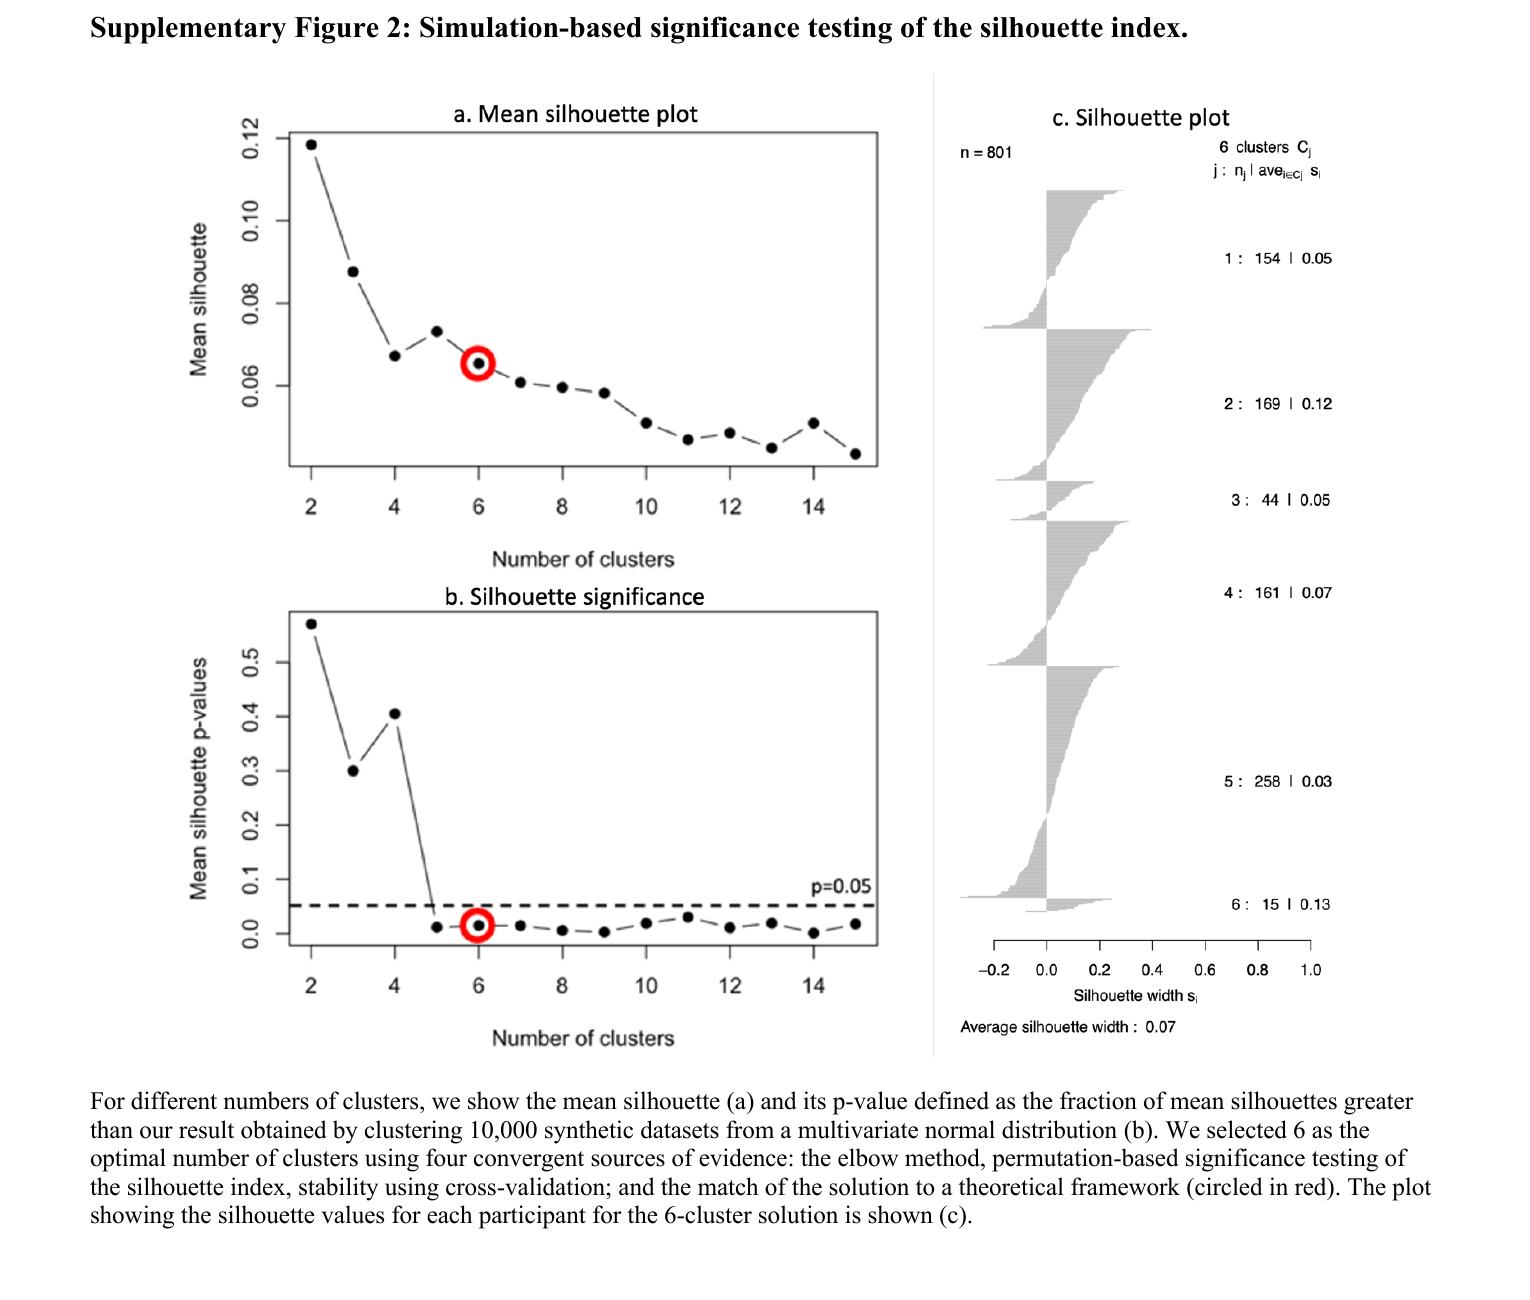
\includegraphics[width=\linewidth,height=.68\textheight,keepaspectratio]{figures/tozzi_supp_fig2.png}\par
    \sourceNote{Original supplementary panel; six clusters circled in red.}
  \end{column}
  \begin{column}{.325\textwidth}
    \centering\paneltitle{FOR2107 · k = 6}\par\vspace{.08cm}
    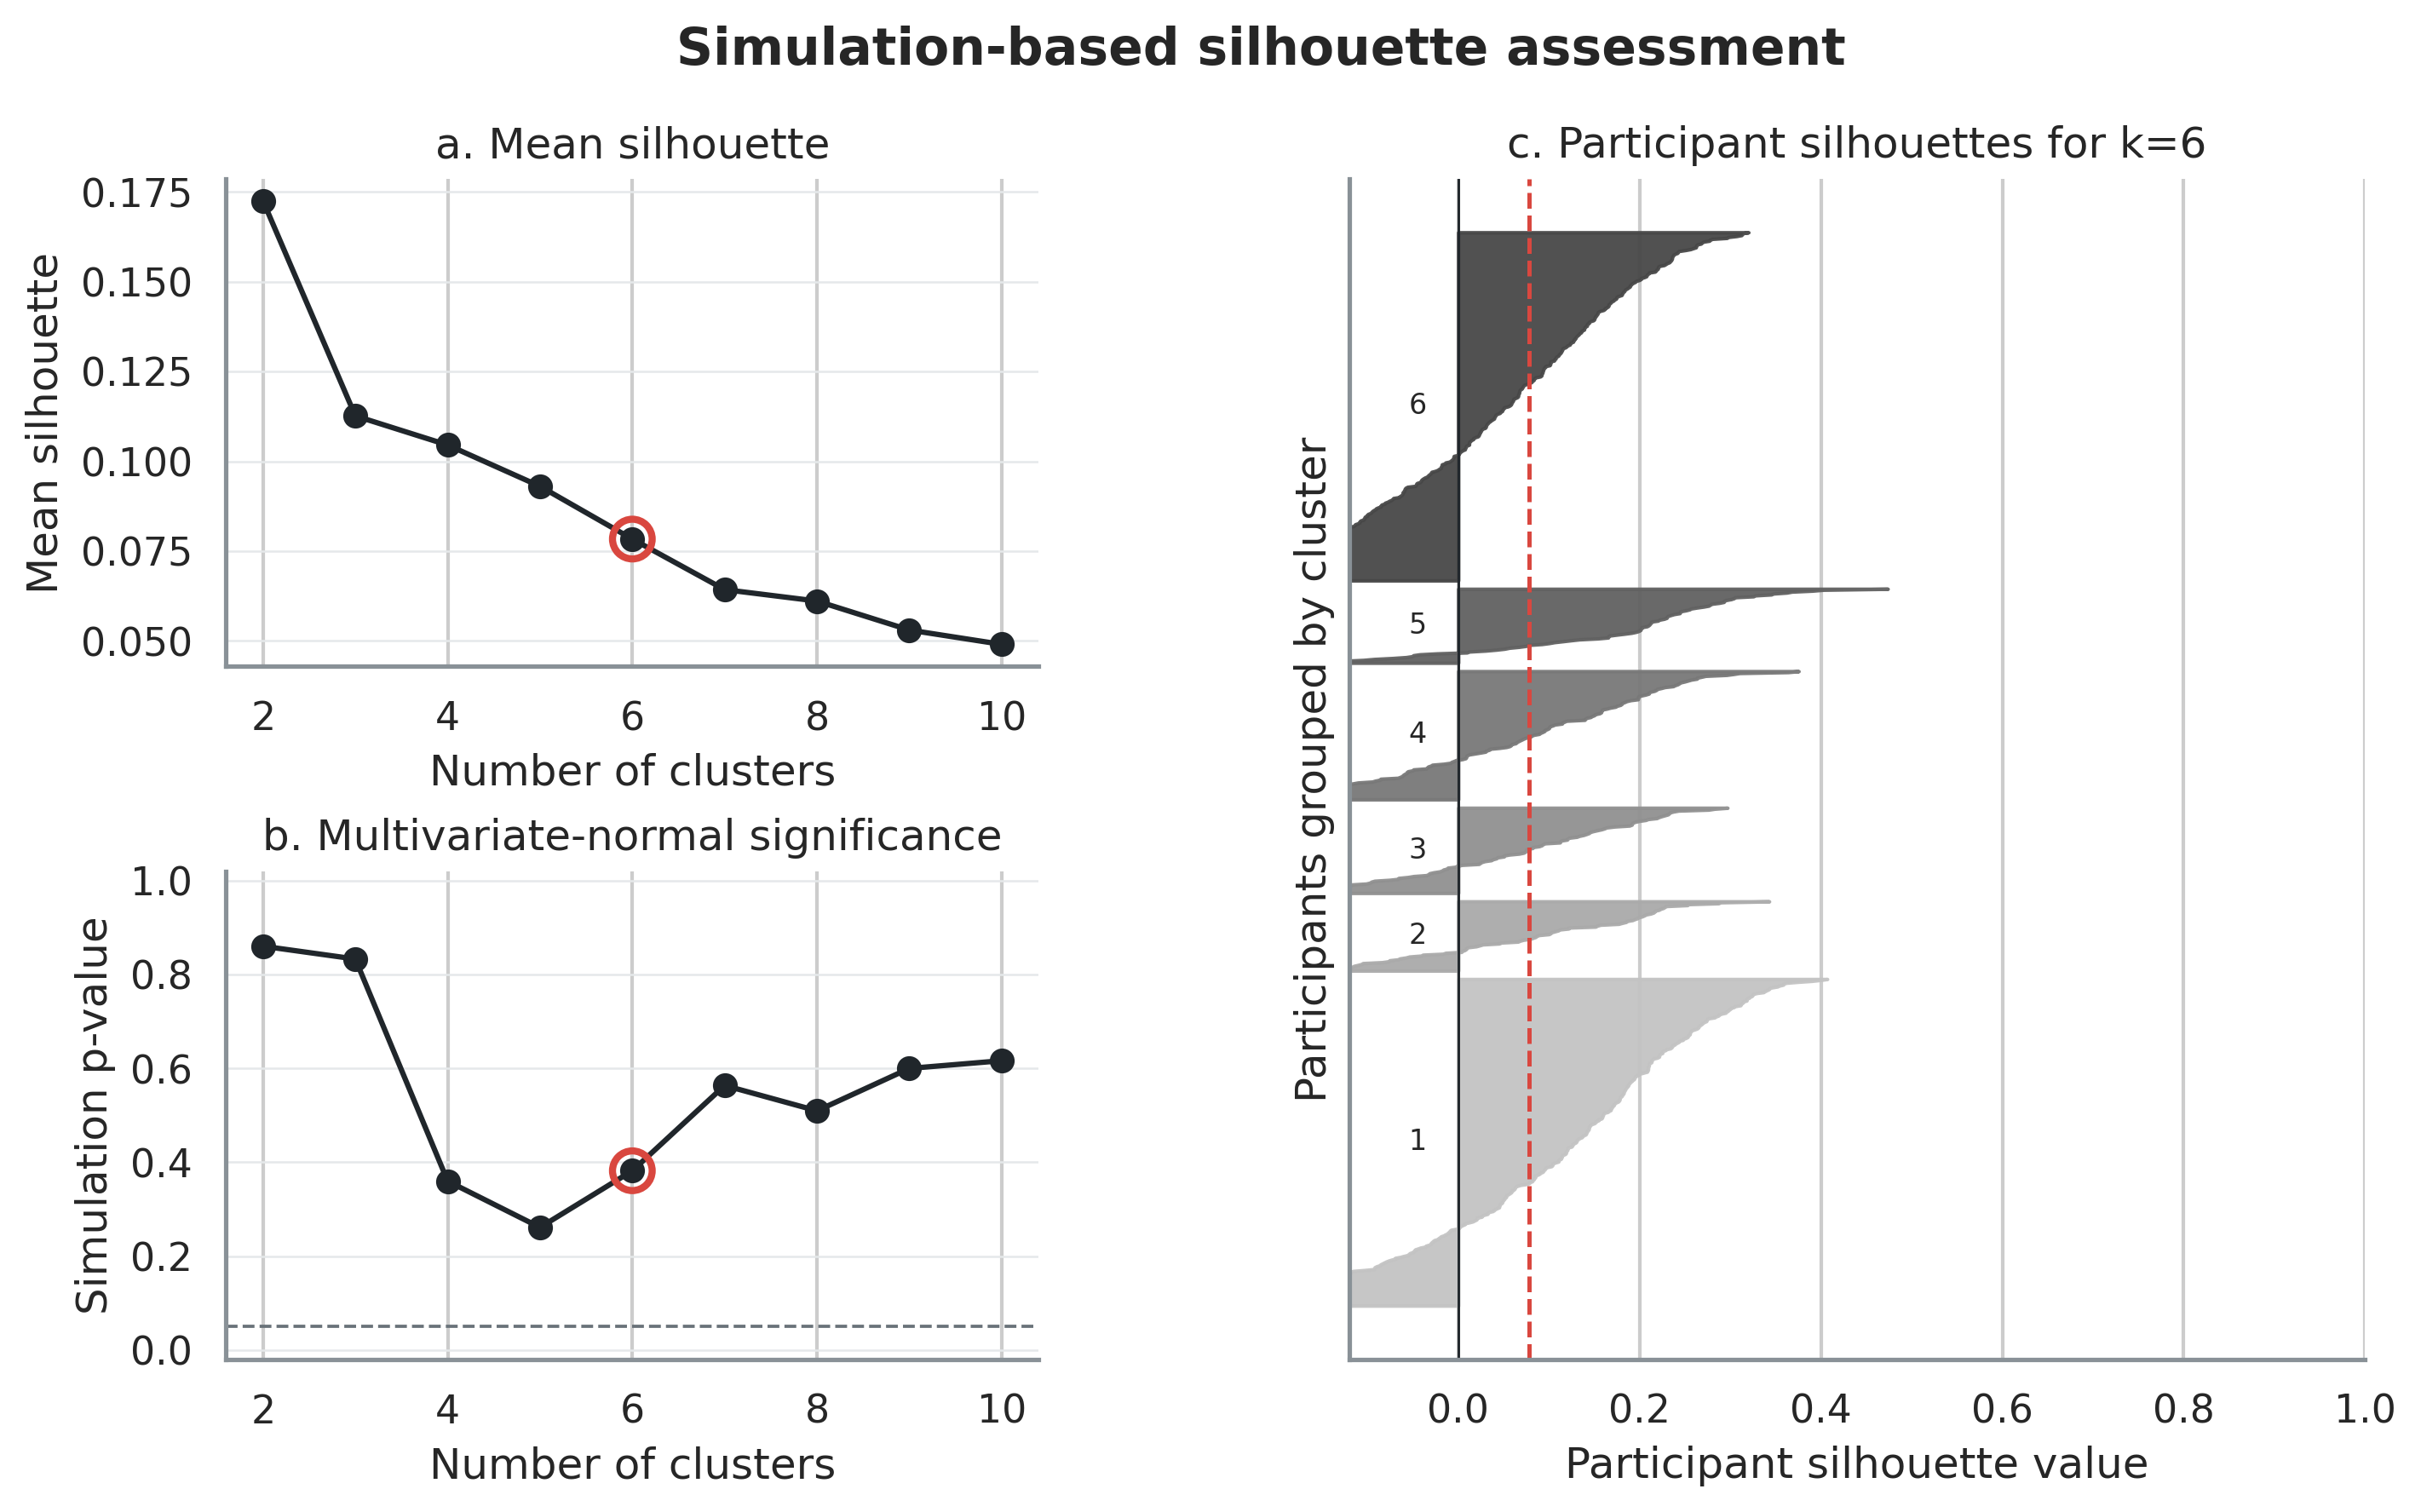
\includegraphics[width=\linewidth,height=.68\textheight,keepaspectratio]{figures/supplementary_figure_2_k6.png}\par
    \sourceNote{14 resting-state edges; k=6 marked as the requested comparison.}
  \end{column}
  \begin{column}{.325\textwidth}
    \centering\paneltitle{FOR2107 · k = 5}\par\vspace{.08cm}
    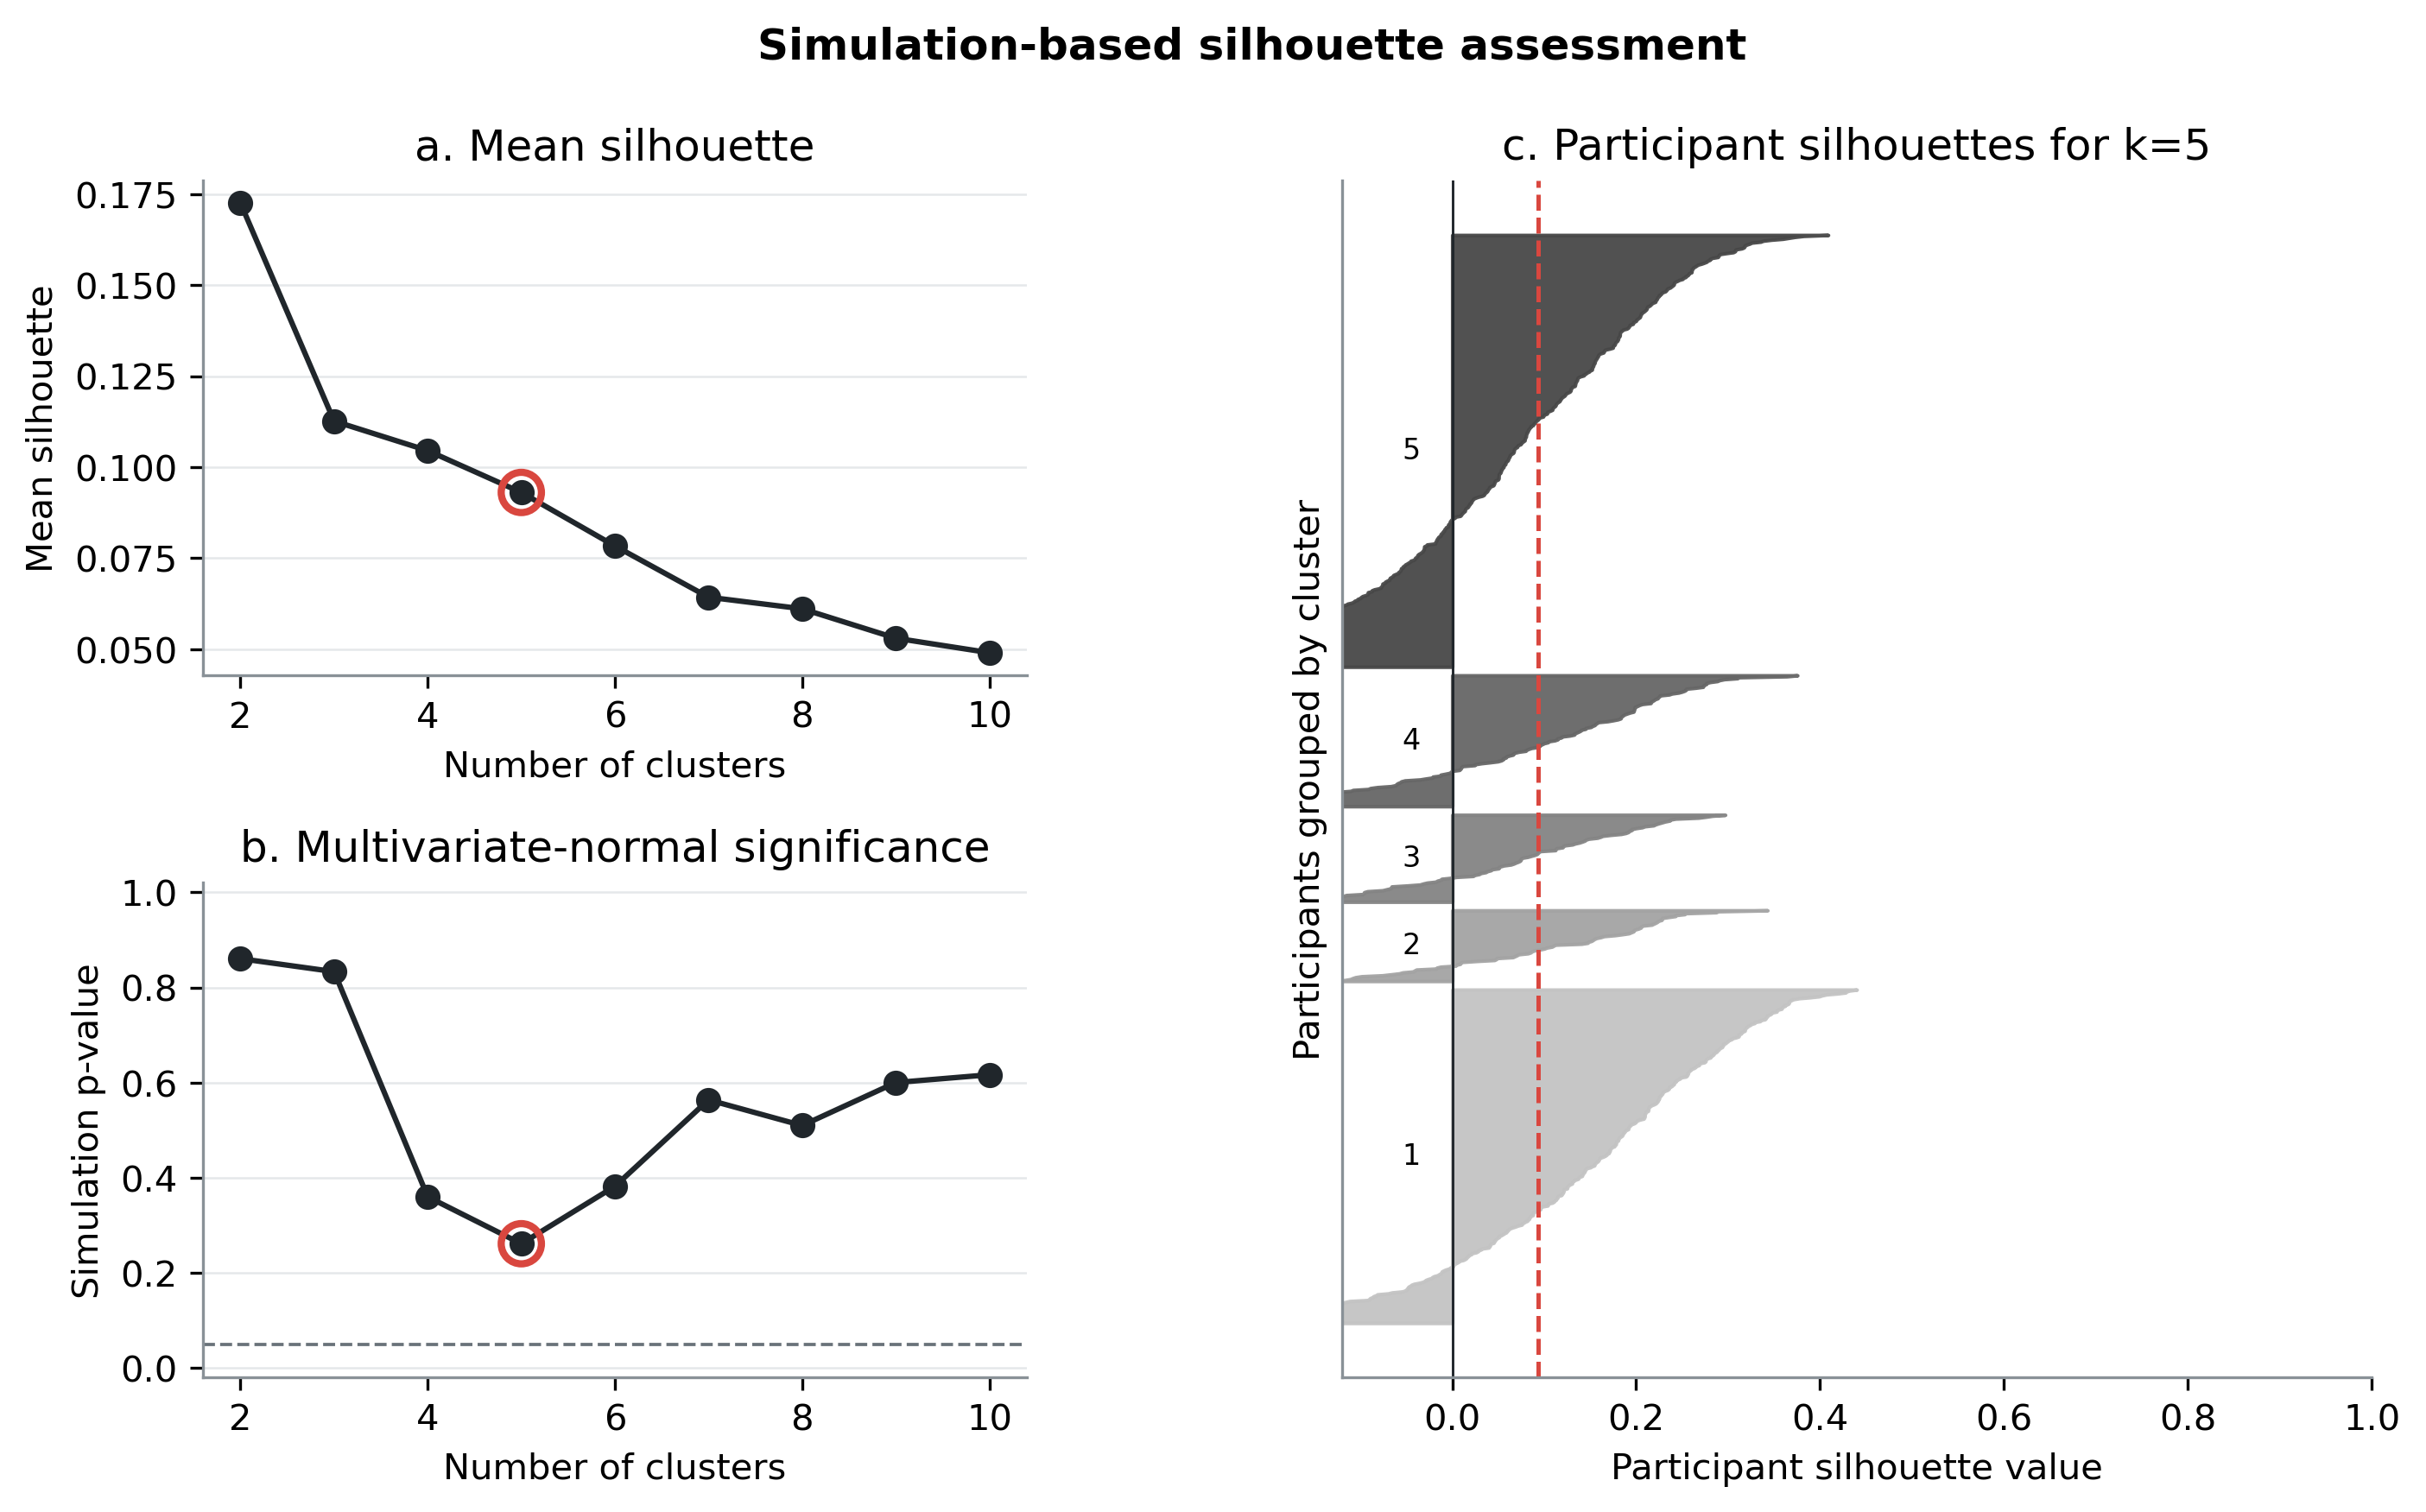
\includegraphics[width=\linewidth,height=.68\textheight,keepaspectratio]{figures/supplementary_figure_2_k5.png}\par
    \sourceNote{Same participants and features; hierarchy cut at five groups.}
  \end{column}
\end{columns}
\vspace{.04cm}
\begin{beamercolorbox}[rounded=true,sep=.15cm,wd=.96\textwidth]{normal text}
\centering\small\color{Navy}\textbf{Reading this carefully:} our permutation panel is significant because independent feature shuffling destroys real covariance. The covariance-preserving multinormal test is not significant for either requested solution.
\end{beamercolorbox}
\end{frame}

\begin{frame}{Supplementary Figure 5: what do the cluster profiles look like?}
\centering
\begin{columns}[T,onlytextwidth]
  \begin{column}{.325\textwidth}
    \centering\paneltitle{Tozzi et al.}\par\vspace{.06cm}
    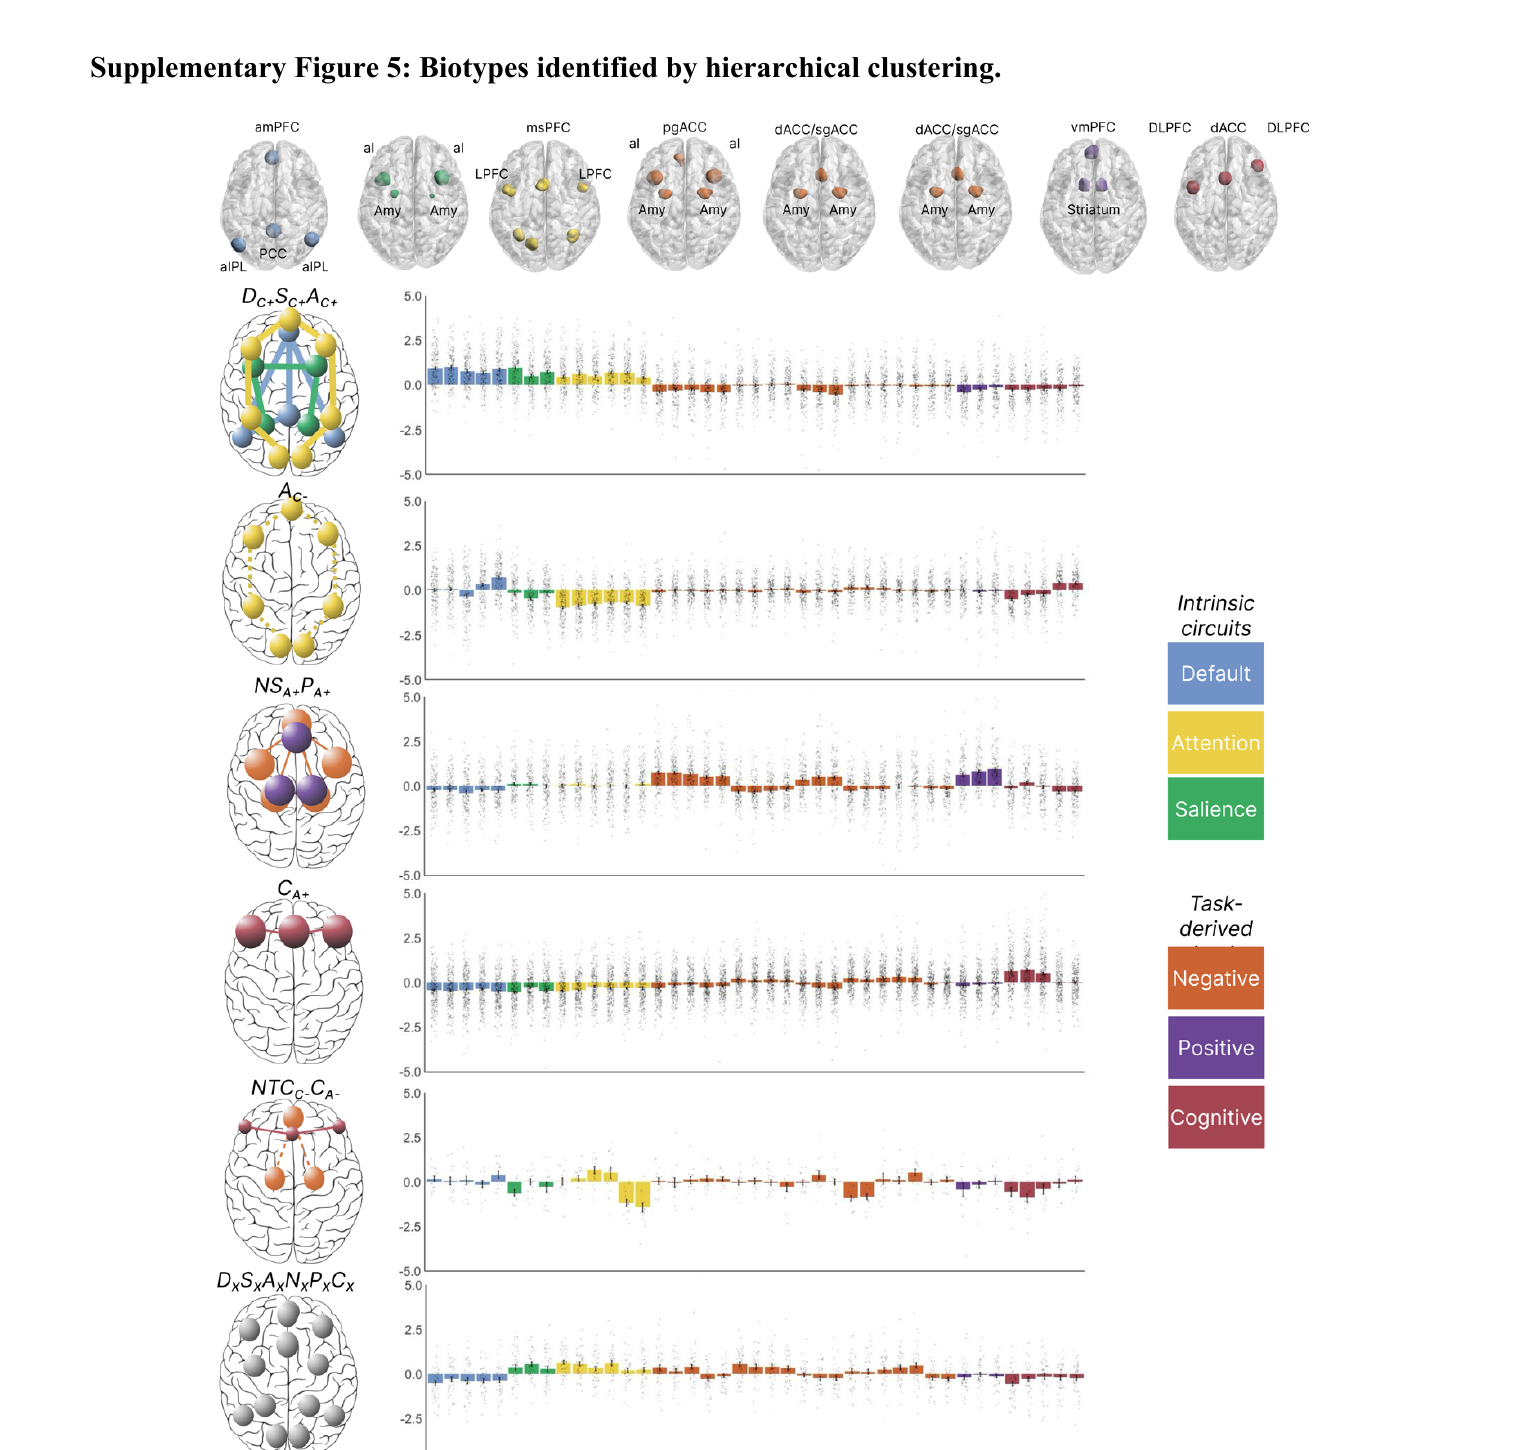
\includegraphics[width=\linewidth,height=.75\textheight,keepaspectratio]{figures/tozzi_supp_fig5.png}\par
    \sourceNote{Original multimodal profiles: rest, task connectivity and task activity.}
  \end{column}
  \begin{column}{.325\textwidth}
    \centering\paneltitle{FOR2107 · k = 6}\par\vspace{.06cm}
    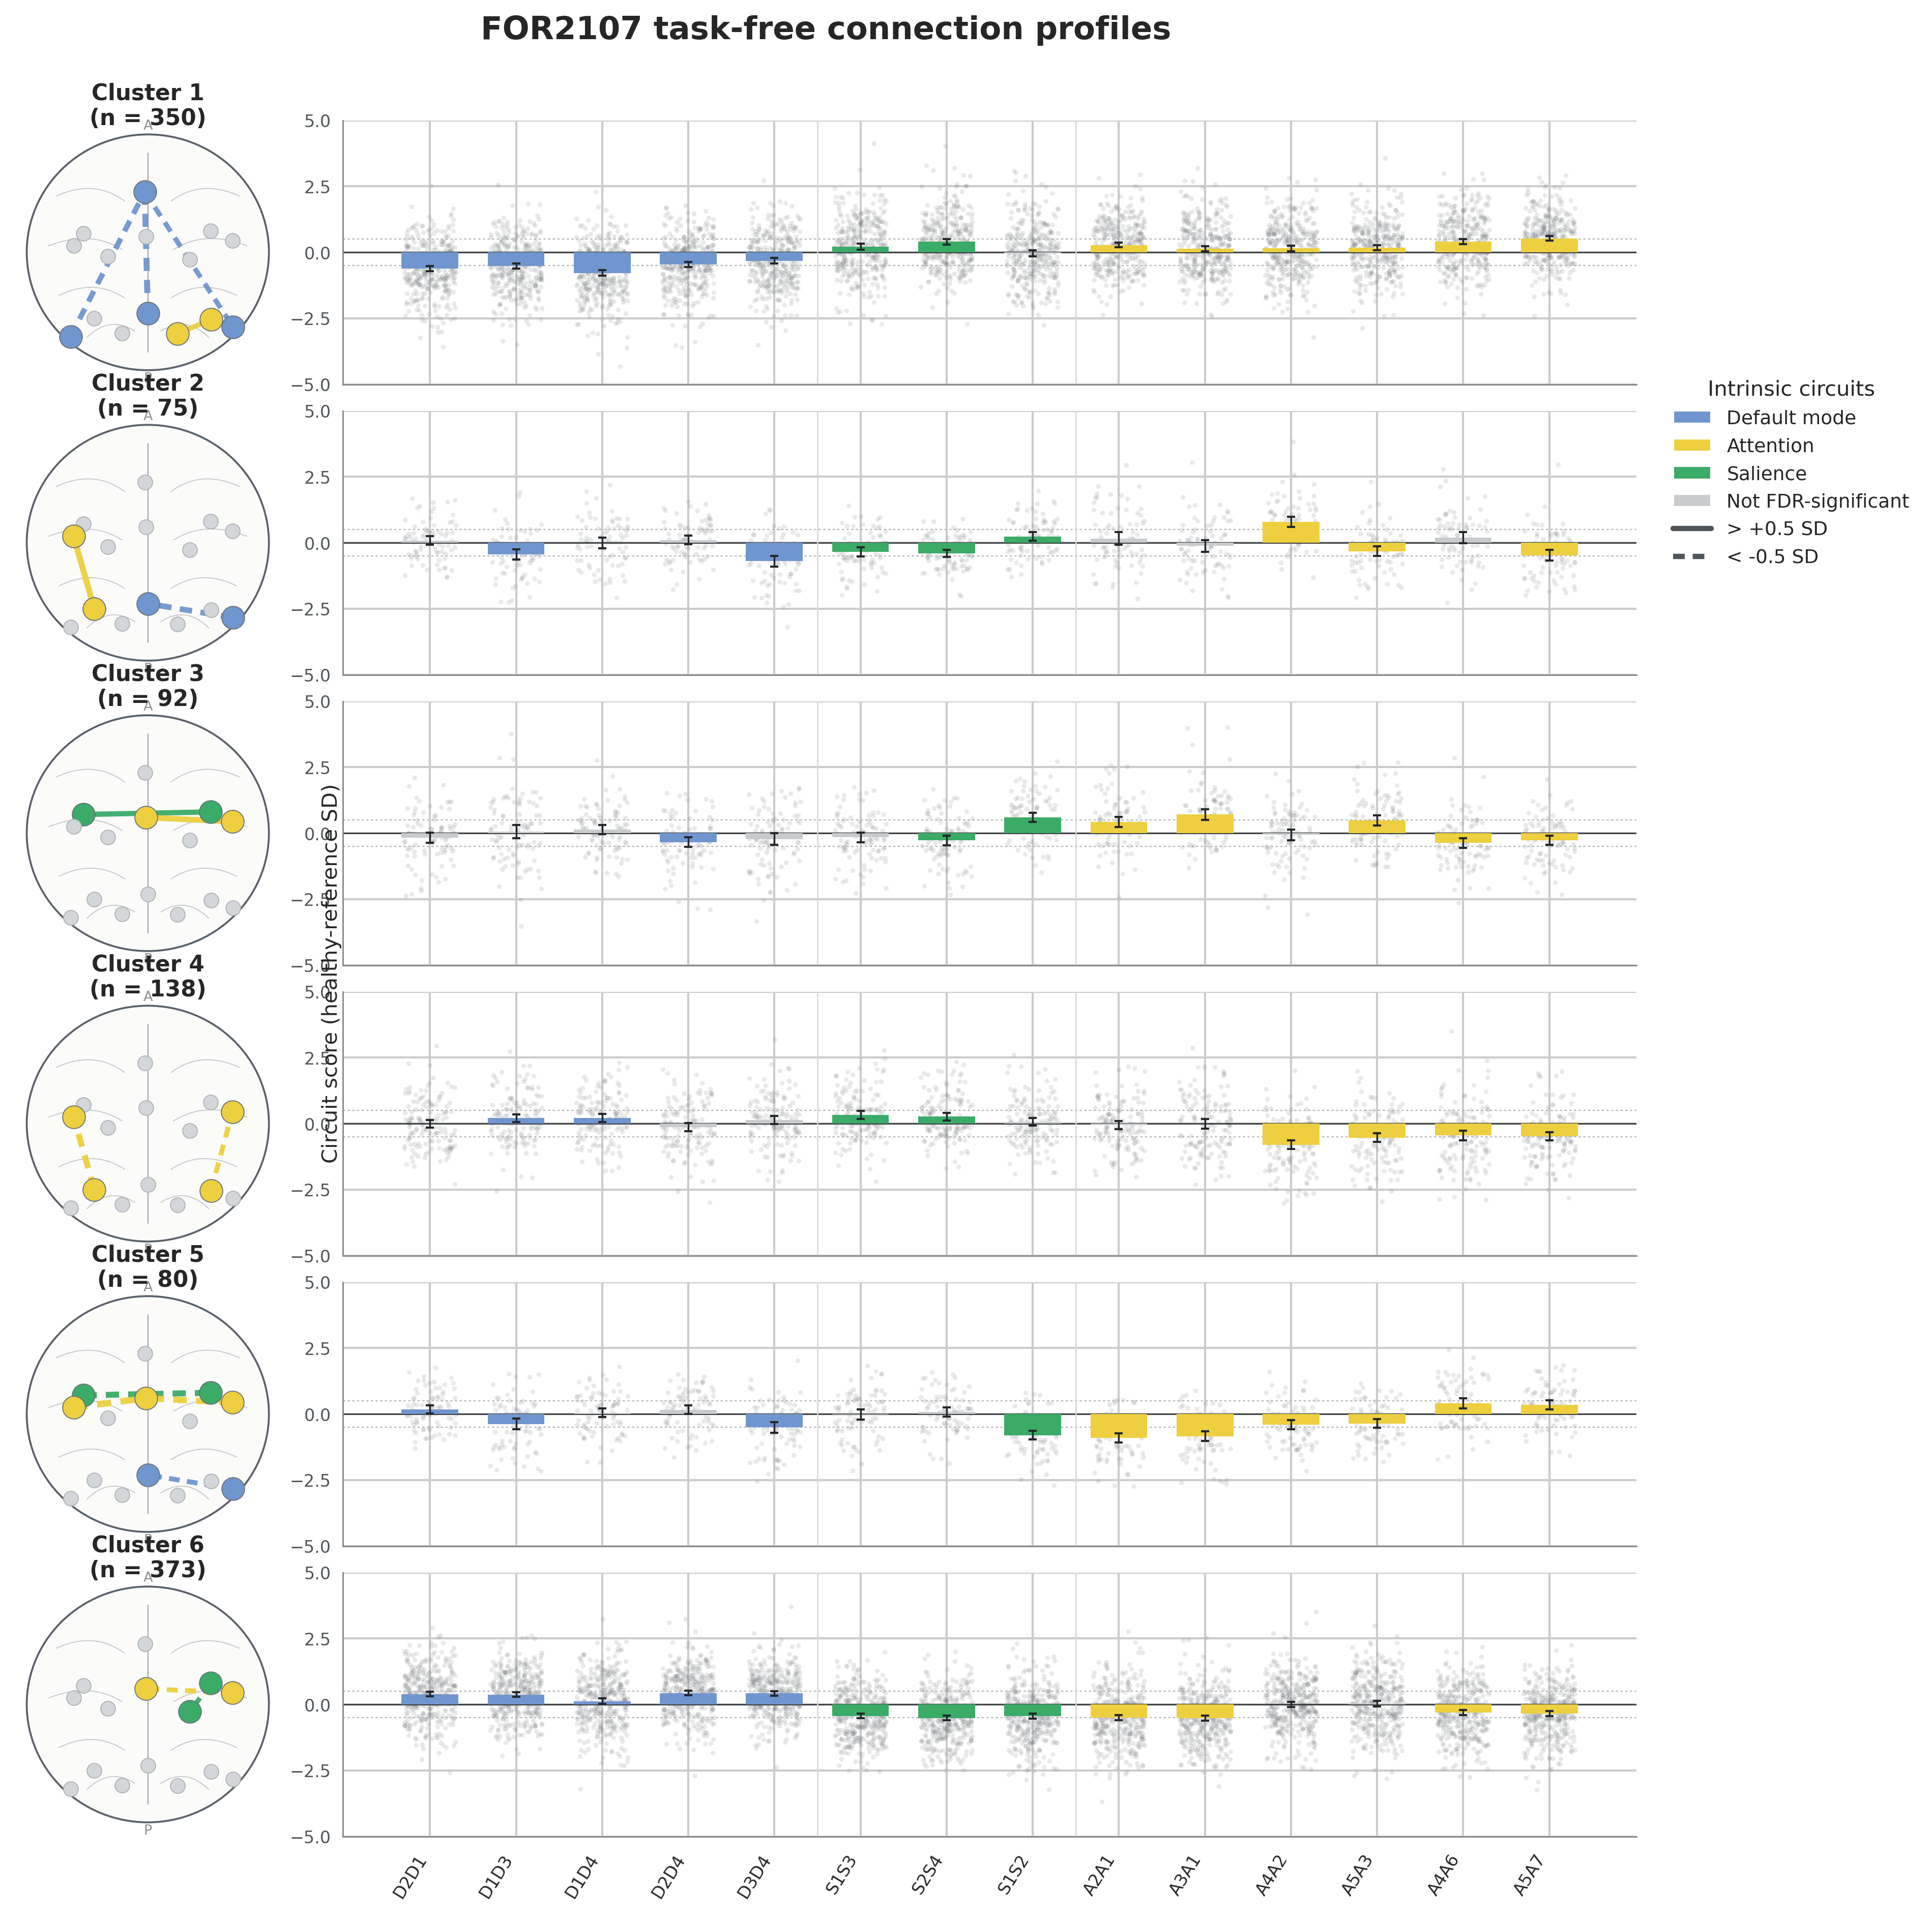
\includegraphics[width=\linewidth,height=.75\textheight,keepaspectratio]{figures/tozzi_style_k6.png}\par
    \sourceNote{Resting-state connectivity only; gray bars are not FDR-significant.}
  \end{column}
  \begin{column}{.325\textwidth}
    \centering\paneltitle{FOR2107 · k = 5}\par\vspace{.06cm}
    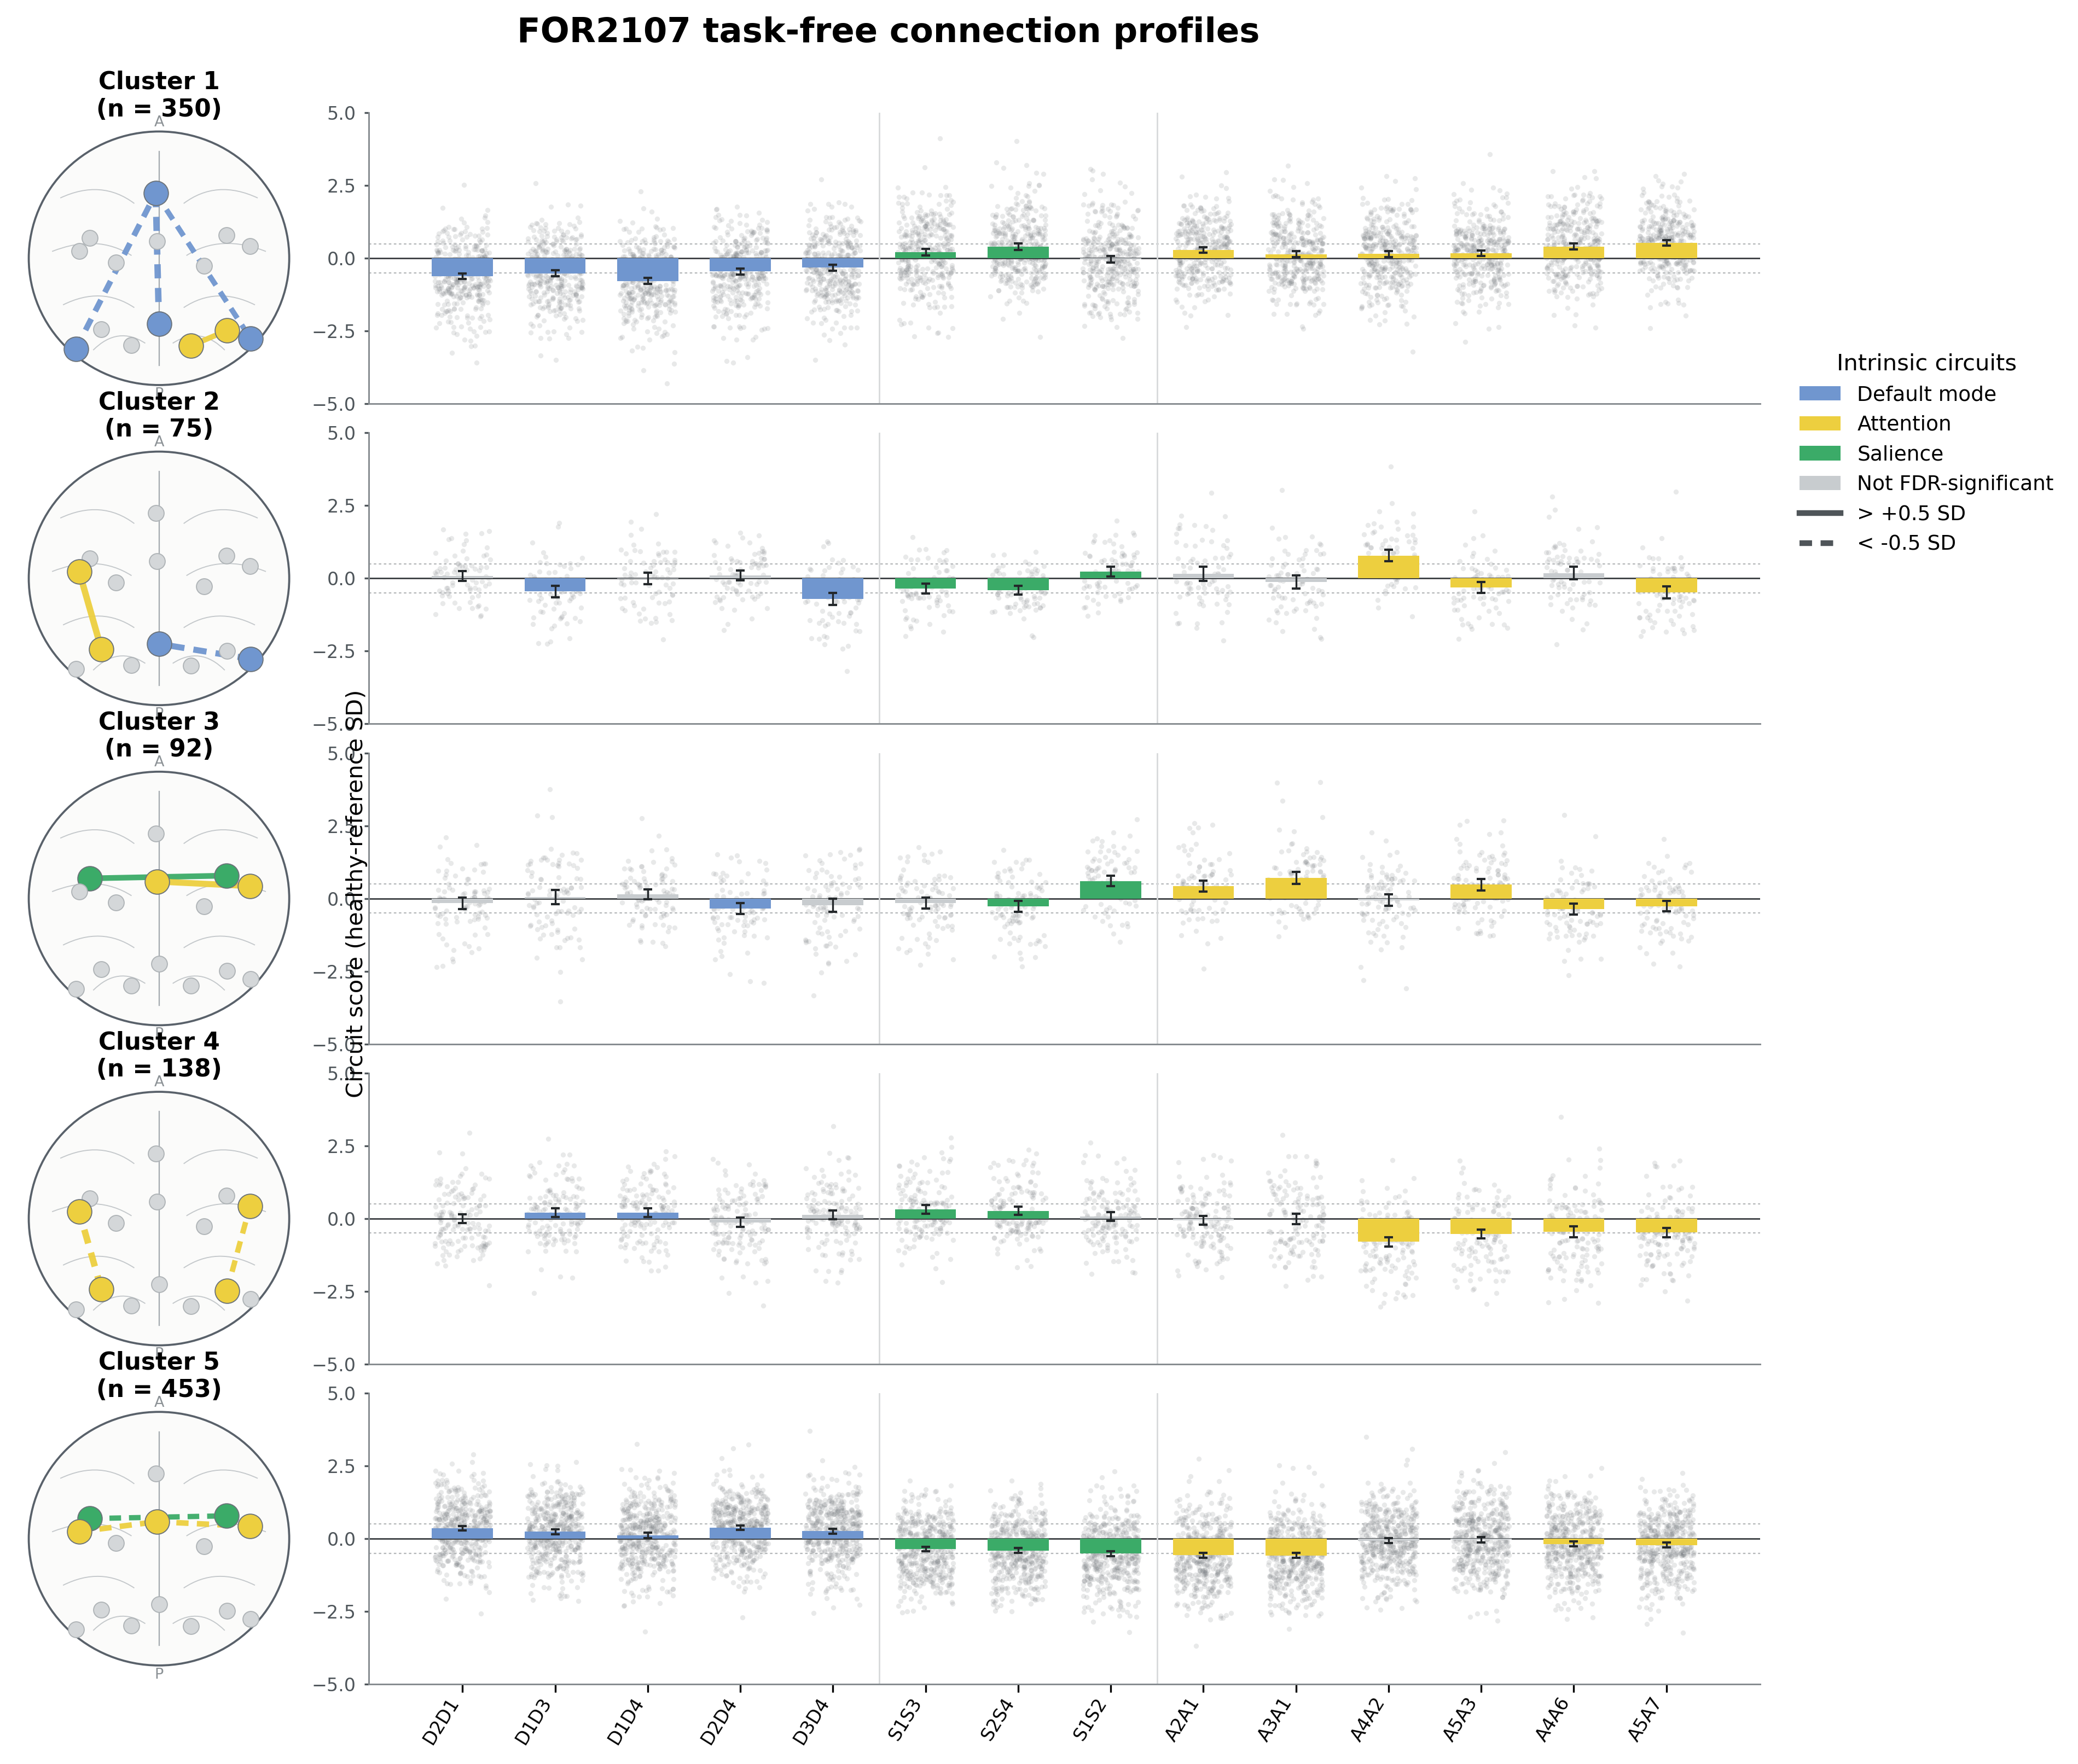
\includegraphics[width=\linewidth,height=.75\textheight,keepaspectratio]{figures/tozzi_style_k5.png}\par
    \sourceNote{Resting-state connectivity only; same anatomical ROI geometry.}
  \end{column}
\end{columns}
\end{frame}

\begin{frame}{What this comparison supports—and what it does not}
\begin{columns}[T,onlytextwidth]
  \begin{column}{.48\textwidth}
    \begin{beamercolorbox}[rounded=true,sep=.25cm,wd=\linewidth]{normal text}
      \color{Teal}\bfseries What is already comparable\par\vspace{.12cm}
      \small
      \begin{itemize}\setlength\itemsep{.34em}
        \item Correlation-distance, average-linkage hierarchy.
        \item Healthy-reference standardized circuit scores.
        \item Elbow, silhouette, permutation, resampling and split-half diagnostics.
        \item Anatomically matched Tozzi ROI definitions for the 14 rest edges.
      \end{itemize}
    \end{beamercolorbox}
  \end{column}
  \begin{column}{.48\textwidth}
    \begin{beamercolorbox}[rounded=true,sep=.25cm,wd=\linewidth]{normal text}
      \color{Red}\bfseries What remains unresolved\par\vspace{.12cm}
      \small
      \begin{itemize}\setlength\itemsep{.34em}
        \item No evidence that k=5 or k=6 beats a covariance-preserving null.
        \item No task-derived activity/connectivity features yet.
        \item No Go/NoGo equivalent and no independent clinical replication.
        \item Cluster profiles are descriptive patterns, not validated biotypes.
      \end{itemize}
    \end{beamercolorbox}
  \end{column}
\end{columns}
\vfill

\begin{tikzpicture}
  \fill[Wash,rounded corners=4pt] (0,0) rectangle (14.6,.88);
  \node[anchor=west,text width=14.1cm] at (.28,.44) {\color{Navy}\small\textbf{Current assessment:} the figures reproduce the visual analysis framework, but the resting-only data do not yet justify selecting a biological cluster count.};
\end{tikzpicture}
\vspace{.12cm}
\sourceNote{Original paper panels are reproduced from the local supplementary PDF for scientific discussion; current panels are generated from repository outputs.}
\end{frame}

\end{document}
